% ============================================================================
% Deliverable 2 - Generative Artificial Intelligence (580694), Primavera 2026
% Documento tecnico: UNA pagina vertical.
%
% Las cifras NO se escriben a mano: salen de results_d2/ via
%     python report/fill_d2.py results_d2 results_d2_holdout
% que genera report/d2_numbers.tex. Compilar:  pdflatex deliverable2_es.tex (x2)
% Version en UN solo archivo (cifras incluidas) para Overleaf: Deliverable2_overleaf.tex
% ============================================================================
% ############################################################################
% ###  EDITA SOLO ESTAS 3 LINEAS (lo que va dentro de las llaves { })      ###
% ###  En los links: _ se escribe \_   % se escribe \%   & se escribe \&    ###
% ############################################################################
\newcommand{\EQUIPO}{Nombre Apellido \textbullet\ Nombre Apellido \textbullet\ Nombre Apellido}
\newcommand{\REPO}{github.com/usuario/repositorio}
\newcommand{\VIDEO}{youtu.be/XXXXXXXX}
% ############################################################################

\documentclass[10pt,a4paper]{extarticle}

\usepackage[utf8]{inputenc}
\usepackage[T1]{fontenc}
\usepackage[margin=0.8cm,top=0.6cm,bottom=0.4cm]{geometry}
\usepackage{helvet}\renewcommand{\familydefault}{\sfdefault}
\usepackage{xcolor}
\usepackage{multicol}
\usepackage{booktabs}
\usepackage{enumitem}
\usepackage{tcolorbox}
\usepackage{pgfplots}
\usepackage{tikz}
\usepackage{microtype}
\pgfplotsset{compat=1.16}
\usetikzlibrary{arrows.meta,positioning,fit,calc}
\tcbuselibrary{skins}

\hyphenpenalty=10000 \exhyphenpenalty=10000 \tolerance=3000 \emergencystretch=2.5em

\definecolor{navy}{HTML}{16314F}
\definecolor{steel}{HTML}{3C5A80}
\definecolor{amber}{HTML}{B45309}
\definecolor{crimson}{HTML}{9B1C1C}
\definecolor{teal}{HTML}{0F766E}
\definecolor{paper}{HTML}{F4F6F9}
\definecolor{rule}{HTML}{C9D2DE}
\definecolor{note}{HTML}{FDF3D8}
\definecolor{mint}{HTML}{E6F4F1}

\setlength{\parindent}{0pt}
\setlength{\columnsep}{6mm}
\setlength{\multicolsep}{2pt}
\setlength{\parskip}{0.5mm}
\pagestyle{empty}

\newcommand{\ph}[1]{\colorbox{yellow!60}{\textcolor{black}{\textbf{#1}}}}
% GENERADO por report/fill_d2.py -- no editar a mano.
\newcommand{\accBase}{28{,}0}
\newcommand{\accBaseH}{40{,}0}
\newcommand{\accCot}{28{,}0}
\newcommand{\accHeur}{54{,}0}
\newcommand{\accHeurH}{76{,}0}
\newcommand{\accPerm}{30{,}0}
\newcommand{\accScal}{42{,}0}
\newcommand{\accSone}{58{,}0}
\newcommand{\accStruct}{20{,}0}
\newcommand{\accStwo}{48{,}0}
\newcommand{\accStwoH}{58{,}0}
\newcommand{\agreeSone}{48}
\newcommand{\agreeStwo}{42}
\newcommand{\callsBase}{1{,}0}
\newcommand{\callsCot}{1{,}0}
\newcommand{\callsHeur}{0{,}0}
\newcommand{\callsPerm}{4{,}0}
\newcommand{\callsScal}{5{,}2}
\newcommand{\callsSone}{5{,}2}
\newcommand{\callsStruct}{1{,}0}
\newcommand{\callsStwo}{5{,}2}
\newcommand{\chiBase}{15{,}8}
\newcommand{\chiCot}{4{,}3}
\newcommand{\chiHeur}{4{,}9}
\newcommand{\chiPBase}{0{,}001}
\newcommand{\chiPCot}{0{,}228}
\newcommand{\chiPHeur}{0{,}181}
\newcommand{\chiPPerm}{0{,}044}
\newcommand{\chiPScal}{0{,}940}
\newcommand{\chiPSone}{0{,}572}
\newcommand{\chiPStruct}{3{,}1\times10^{-14}}
\newcommand{\chiPStwo}{0{,}792}
\newcommand{\chiPerm}{8{,}1}
\newcommand{\chiScal}{0{,}4}
\newcommand{\chiSone}{2{,}0}
\newcommand{\chiStruct}{66{,}0}
\newcommand{\chiStwo}{1{,}0}
\newcommand{\ciBase}{18--42}
\newcommand{\ciBaseH}{28--54}
\newcommand{\ciCot}{18--42}
\newcommand{\ciHeur}{40--67}
\newcommand{\ciHeurH}{63--86}
\newcommand{\ciPerm}{19--44}
\newcommand{\ciScal}{29--56}
\newcommand{\ciSone}{44--71}
\newcommand{\ciStruct}{11--33}
\newcommand{\ciStwo}{35--62}
\newcommand{\ciStwoH}{44--71}
\newcommand{\constOne}{80/122}
\newcommand{\diffBase}{6/17 $\cdot$ 6/17 $\cdot$ 2/16}
\newcommand{\diffCot}{4/17 $\cdot$ 5/17 $\cdot$ 5/16}
\newcommand{\diffHeur}{7/17 $\cdot$ 7/17 $\cdot$ 13/16}
\newcommand{\diffPerm}{6/17 $\cdot$ 6/17 $\cdot$ 3/16}
\newcommand{\diffScal}{5/17 $\cdot$ 6/17 $\cdot$ 10/16}
\newcommand{\diffSone}{9/17 $\cdot$ 7/17 $\cdot$ 13/16}
\newcommand{\diffStruct}{3/17 $\cdot$ 4/17 $\cdot$ 3/16}
\newcommand{\diffStwo}{8/17 $\cdot$ 7/17 $\cdot$ 9/16}
\newcommand{\factAcc}{60{,}7}
\newcommand{\factPairs}{122}
\newcommand{\factRight}{74}
\newcommand{\fcAtk}{Electric}
\newcommand{\fcChosen}{MOVE\_1 (Thunderbolt)}
\newcommand{\fcDef}{Ground}
\newcommand{\fcDiff}{MEDIUM}
\newcommand{\fcEnemy}{Ground}
\newcommand{\fcFixed}{s\'i}
\newcommand{\fcId}{32}
\newcommand{\fcIdOrQ}{32}
\newcommand{\fcIsModern}{0}
\newcommand{\fcModel}{1}
\newcommand{\fcOptimal}{MOVE\_3 (Razor Leaf)}
\newcommand{\fcPlayer}{Water}
\newcommand{\fcRegret}{100}
\newcommand{\fcSaid}{normal damage}
\newcommand{\fcTable}{MOVE\_1 & Thunderbolt & Electric & \textcolor{crimson}{\textbf{$\times$1}} & $\times$0 & \textcolor{crimson}{\textbf{95{,}0}} & 0{,}0\\
MOVE\_2 & Strength & Normal & $\times$1 & $\times$1 & 80{,}0 & 80{,}0\\
MOVE\_3 & Razor Leaf & Grass & \textcolor{crimson}{\textbf{$\times$1}} & $\times$2 & \textcolor{crimson}{\textbf{52{,}2}} & 104{,}5\\
MOVE\_4 & Psybeam & Psychic & $\times$1 & $\times$1 & 65{,}0 & 65{,}0\\}
\newcommand{\fcTruth}{0}
\newcommand{\genBullet}{Ninguno de sus 48 errores es el valor de Gen~II+: no confunde generaciones.}
\newcommand{\hasFailure}{1}
\newcommand{\holdN}{50}
\newcommand{\holdSeed}{20260927}
\newcommand{\hw}{Tesla T4, float32}
\newcommand{\hwH}{Tesla T4, float32}
\newcommand{\hwNote}{B0, A1, A2, A3, S1, S1$^{+}$ (50 originales) corrieron antes en CPU, float32.}
\newcommand{\libs}{torch 2.11.0+cu128, transformers 5.16.1}
\newcommand{\lossBase}{--}
\newcommand{\lossCot}{10}
\newcommand{\lossHeur}{3}
\newcommand{\lossPerm}{1}
\newcommand{\lossSH}{5}
\newcommand{\lossScal}{4}
\newcommand{\lossSone}{2}
\newcommand{\lossStruct}{7}
\newcommand{\lossStwo}{3}
\newcommand{\lossStwoH}{5}
\newcommand{\modelId}{Qwen/Qwen2.5-1.5B-Instruct}
\newcommand{\modelRev}{989aa7980e}
\newcommand{\nFail}{26}
\newcommand{\nFailFixed}{26}
\newcommand{\nParams}{1{,}54}
\newcommand{\nSameSuper}{5}
\newcommand{\nStates}{50}
\newcommand{\nWrongFacts}{48}
\newcommand{\neutralPct}{87}
\newcommand{\neutralShare}{106/122}
\newcommand{\neutralShareH}{105/117}
\newcommand{\nonNeutral}{2/16}
\newcommand{\nonNeutralH}{1/12}
\newcommand{\pBase}{--}
\newcommand{\pCot}{0{,}092}
\newcommand{\pHeur}{0{,}004}
\newcommand{\pPerm}{1{,}000}
\newcommand{\pSH}{0{,}453}
\newcommand{\pScal}{0{,}118}
\newcommand{\pSone}{7{,}3\times10^{-4}}
\newcommand{\pStruct}{0{,}344}
\newcommand{\pStwo}{0{,}021}
\newcommand{\pStwoH}{0{,}064}
\newcommand{\permComplete}{49}
\newcommand{\posBase}{(MOVE\_1,14)(MOVE\_2,23)(MOVE\_3,9)(MOVE\_4,4)}
\newcommand{\posCot}{(MOVE\_1,11)(MOVE\_2,17)(MOVE\_3,7)(MOVE\_4,13)}
\newcommand{\posHeur}{(MOVE\_1,18)(MOVE\_2,12)(MOVE\_3,7)(MOVE\_4,13)}
\newcommand{\posOpt}{(MOVE\_1,18)(MOVE\_2,8)(MOVE\_3,14)(MOVE\_4,10)}
\newcommand{\posPerm}{(MOVE\_1,14)(MOVE\_2,20)(MOVE\_3,7)(MOVE\_4,9)}
\newcommand{\posScal}{(MOVE\_1,14)(MOVE\_2,13)(MOVE\_3,11)(MOVE\_4,12)}
\newcommand{\posSone}{(MOVE\_1,16)(MOVE\_2,12)(MOVE\_3,9)(MOVE\_4,13)}
\newcommand{\posStruct}{(MOVE\_1,1)(MOVE\_2,37)(MOVE\_3,4)(MOVE\_4,8)}
\newcommand{\posStwo}{(MOVE\_1,13)(MOVE\_2,15)(MOVE\_3,10)(MOVE\_4,12)}
\newcommand{\priorHalf}{0{,}90}
\newcommand{\recallHalf}{0/21}
\newcommand{\recallOne}{72/80}
\newcommand{\recallTwo}{2/18}
\newcommand{\recallZero}{0/3}
\newcommand{\regretBase}{0{,}33}
\newcommand{\regretCot}{0{,}36}
\newcommand{\regretHeur}{0{,}22}
\newcommand{\regretPerm}{0{,}32}
\newcommand{\regretScal}{0{,}30}
\newcommand{\regretSone}{0{,}19}
\newcommand{\regretStruct}{0{,}42}
\newcommand{\regretStwo}{0{,}25}
\newcommand{\runMinutes}{113}
\newcommand{\sOneModal}{0{,}5}
\newcommand{\sOneModalProb}{0{,}97}
\newcommand{\sOneModalShare}{122/122}
\newcommand{\sameMove}{8}
\newcommand{\sameSlot}{0}
\newcommand{\sameSuper}{El\'ectrico--El\'ectrico, Veneno--Veneno, Ps\'iquico--Ps\'iquico, Roca--Roca, Agua--Agua}
\newcommand{\secsBase}{5{,}3}
\newcommand{\secsBaseH}{0{,}33}
\newcommand{\secsCot}{96{,}9}
\newcommand{\secsHeur}{0{,}0}
\newcommand{\secsPerm}{15{,}1}
\newcommand{\secsScal}{0{,}0}
\newcommand{\secsSone}{12{,}6}
\newcommand{\secsStruct}{5{,}8}
\newcommand{\secsStwo}{0{,}3}
\newcommand{\secsStwoH}{0{,}10}
\newcommand{\seed}{20260830}
\newcommand{\split}{17/17/16}
\newcommand{\strictBase}{100}
\newcommand{\strictCot}{56}
\newcommand{\strictHeur}{100}
\newcommand{\strictPerm}{100}
\newcommand{\strictScal}{100}
\newcommand{\strictSone}{100}
\newcommand{\strictStruct}{100}
\newcommand{\strictStwo}{100}
\newcommand{\ties}{3}
\newcommand{\unparsed}{0}
\newcommand{\verdictSH}{\textbf{El modelo no aporta sobre ignorar los tipos:} frente a H, S2 gana en 2 estados y pierde en 5 ($p=0{,}453$). En los 50 estados nuevos es \emph{peor}: gana en 0, pierde en 9 ($p=0{,}004$). Sus hechos de tipos valen menos que asumir $\times$1.}
\newcommand{\winBase}{--}
\newcommand{\winCot}{3}
\newcommand{\winHeur}{16}
\newcommand{\winPerm}{2}
\newcommand{\winSH}{2}
\newcommand{\winScal}{11}
\newcommand{\winSone}{17}
\newcommand{\winStruct}{3}
\newcommand{\winStwo}{13}
\newcommand{\winStwoH}{14}


\newcommand{\heading}[1]{%
  \par\vspace{1.2mm}\noindent
  {\color{navy}\bfseries\small\MakeUppercase{#1}}\par\vspace{0.5mm}
  {\color{amber}\hrule height 1pt}\vspace{0.9mm}\noindent\ignorespaces}

\newtcolorbox{keybox}[1]{colback=note,colframe=amber,boxrule=0.7pt,
  left=1.6mm,right=1.6mm,top=1.1mm,bottom=1.1mm,arc=1mm,
  fonttitle=\bfseries\footnotesize,coltitle=white,colbacktitle=amber,title={#1}}
\newtcolorbox{failbox}[1]{colback=white,colframe=crimson,boxrule=0.7pt,
  left=1.6mm,right=1.6mm,top=1.1mm,bottom=1.1mm,arc=1mm,
  fonttitle=\bfseries\footnotesize,coltitle=white,colbacktitle=crimson,title={#1}}
\setlist[itemize]{leftmargin=3.4mm,itemsep=0.35mm,topsep=0.5mm,parsep=0pt}

\begin{document}
\small

% ================================================================ CABECERA ==
\begin{tcolorbox}[colback=navy,colframe=navy,boxrule=0pt,left=3mm,right=3mm,top=1.6mm,bottom=1.6mm,arc=1mm]
{\color{white}\bfseries\Large Descomponer para decidir: un modelo de 1{,}5B juega Pok\'emon Blue}\\[0.9mm]
{\color{white!85}\normalsize Deliverable 2 \,--\, del diagn\'ostico a un sistema que funciona}\hfill
{\color{white!75}\footnotesize Generative Artificial Intelligence (580694) \textbullet\ Primavera 2026 \textbullet\ UdeC}\\[1.3mm]
{\footnotesize\color{white!85}Equipo:} {\footnotesize\bfseries\color{white}\EQUIPO}\hfill
{\footnotesize\color{white!85}Repo:} {\footnotesize\color{white}\texttt{\REPO}}\hfill
{\footnotesize\color{white!85}Video:} {\footnotesize\color{white}\texttt{\VIDEO}}
\end{tcolorbox}

% ================================================================ PIPELINE ==
\vspace{0.4mm}
{\centering
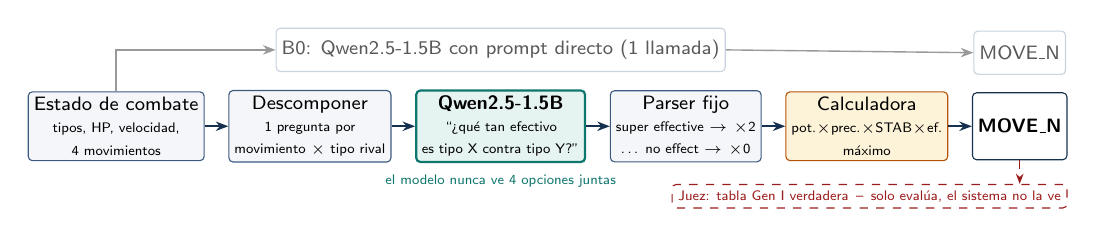
\begin{tikzpicture}[
  font=\scriptsize, node distance=3.2mm and 3.0mm,
  box/.style={draw=steel,fill=paper,rounded corners=1.5pt,align=center,inner sep=2pt,minimum height=8.5mm},
  llm/.style={box,draw=teal,fill=mint,line width=0.8pt},
  tool/.style={box,draw=amber,fill=note},
  obox/.style={box,draw=navy,fill=white,font=\scriptsize\bfseries},
  base/.style={box,draw=rule,fill=white,text=black!65},
  arr/.style={-{Stealth[length=1.6mm]},line width=0.6pt,draw=navy},
  garr/.style={-{Stealth[length=1.6mm]},line width=0.5pt,draw=black!40}]
\node[box] (st) {Estado de combate\\{\tiny tipos, HP, velocidad,}\\{\tiny 4 movimientos}};
\node[box,right=of st] (dec) {Descomponer\\{\tiny 1 pregunta por}\\{\tiny movimiento $\times$ tipo rival}};
\node[llm,right=of dec] (q) {\textbf{Qwen2.5-1.5B}\\{\tiny ``\textquestiondown qu\'e tan efectivo}\\{\tiny es tipo X contra tipo Y?''}};
\node[box,right=of q] (pa) {Parser fijo\\{\tiny super effective $\to\times$2}\\{\tiny \ldots\ no effect $\to\times$0}};
\node[tool,right=of pa] (calc) {Calculadora\\{\tiny pot.$\times$prec.$\times$STAB$\times$ef.}\\{\tiny m\'aximo}};
\node[obox,right=of calc] (mv) {MOVE\_N};
\draw[arr] (st)--(dec); \draw[arr] (dec)--(q); \draw[arr] (q)--(pa); \draw[arr] (pa)--(calc); \draw[arr] (calc)--(mv);
\node[base,above=2.2mm of q,minimum height=5.5mm] (bq) {B0: Qwen2.5-1.5B con prompt directo (1 llamada)};
\node[base,above=2.2mm of mv,minimum height=5.5mm] (bm) {MOVE\_N};
\draw[garr] (st.north) |- (bq.west); \draw[garr] (bq.east) -- (bm.west);
\node[draw=crimson,dashed,rounded corners=1.5pt,below=3.0mm of mv.south east,anchor=north east,font=\tiny,text=crimson,align=center,inner sep=2.2pt]
  (judge) {Juez: tabla Gen I verdadera \,--\, solo eval\'ua, el sistema no la ve};
\draw[-{Stealth[length=1.3mm]},crimson,dashed,line width=0.45pt] (mv.south) -- (mv.south |- judge.north);
\node[font=\tiny,text=teal,below=0.2mm of q.south,anchor=north] {el modelo nunca ve 4 opciones juntas};
\end{tikzpicture}\par}
\vspace{-0.4mm}

\noindent
\begin{minipage}[t]{0.488\linewidth}
\setlength{\parskip}{0.55mm}
% ============================================================ 1. CONTINUIDAD
\heading{1. Continuidad con el D1}
\textbf{Misma tarea, mismo fallo, mismo criterio.} Estado de combate $\to$ \texttt{MOVE\_1}--\texttt{MOVE\_4}; correcto = m\'aximo de potencia $\times$ precisi\'on $\times$ STAB $\times$ efectividad (Gen I). Fallo del D1: con prompt estructurado acertaba 16{,}7\,\%, \emph{bajo el azar}: respond\'ia por posici\'on en vez de combinar los atributos.

\textbf{Desviaciones declaradas.} (i) B0 = prompt directo del D1 + pedir \texttt{MOVE\_N} (amenaza T1 del D1). (ii) \textbf{\nStates} estados, mismo generador y semilla (\seed; con $n{=}30$ reproduce los del D1) + \textbf{\holdN\ nuevos} (semilla \holdSeed).

% ============================================================ 2. MODELO
\heading{2. Modelo elegido}
\textbf{\texttt{\modelId}}, revisi\'on \texttt{\modelRev}, \nParams\,B par\'ametros, Colab \hw\ (\libs). {\scriptsize \hwNote}
\begin{itemize}
\item \textbf{Econom\'ia:} el m\'as peque\~no de los tres candidatos del D1 y el \'unico con un perfil de fallo \emph{medido} en esta tarea.
\item \textbf{Le quita el paso que lo separaba de los otros dos}, razonar en varios pasos (GSM8K: Phi-3.5-mini 86{,}2, Llama-3.2-3B 77{,}7, Qwen 73{,}2): aqu\'i combina la calculadora.
\end{itemize}

% ============================================================ 3. INTERVENCION
\heading{3. La intervenci\'on y su v\'inculo con el fallo}
\textbf{Descomposici\'on + herramienta} (diagrama): \emph{una} pregunta por movimiento usable y tipo rival; el modelo responde con las frases del juego, un parser fijo las traduce a $\times2/\times1/\times0{,}5/\times0$ y la calculadora elige el m\'aximo.
\begin{itemize}
\item \textbf{Ataca el sesgo de posici\'on:} el modelo nunca ve las cuatro opciones juntas.
\item \textbf{Ataca la combinaci\'on:} el modelo aporta hechos sueltos; la aritm\'etica la hace c\'odigo.
\item \textbf{El modelo es la \'unica fuente de tipos:} la soluci\'on no tiene la tabla (lo verifica un test). Referencia \textbf{H}: la misma calculadora con toda efectividad en $\times$1.
\end{itemize}

% ============================================================ 4. ESTRATEGIAS
\heading{4. Estrategias evaluadas ($n = \nStates$, mismos estados)}
{\centering\footnotesize
\begin{tabular}{@{}llrrr@{}}
\toprule
& \textbf{Qu\'e cambia} & \textbf{llam.} & \textbf{ACC [IC 95\%]} & \textbf{vs B0}\\
\midrule
B0 & prompt directo (\textbf{baseline}) & \callsBase & \accBase\,\% [\ciBase] & --\\
A1 & prompt estructurado del D1 & \callsStruct & \accStruct\,\% [\ciStruct] & +\winStruct/--\lossStruct\\
A2 & B0 con 4 \'ordenes + voto & \callsPerm & \accPerm\,\% [\ciPerm] & +\winPerm/--\lossPerm\\
A3 & chain-of-thought + f\'ormula & \callsCot & \accCot\,\% [\ciCot] & +\winCot/--\lossCot\\
S1 & hechos en n\'umeros (v1) & \callsSone & \accSone\,\% [\ciSone] & +\winSone/--\lossSone\\
S1$^{+}$ & S1 calibrada & \callsScal & \accScal\,\% [\ciScal] & +\winScal/--\lossScal\\
H & sin modelo: ignora tipos & 0 & \accHeur\,\% [\ciHeur] & +\winHeur/--\lossHeur\\
\textbf{S2} & \textbf{hechos en palabras} & \callsStwo & \textbf{\accStwo\,\%} [\ciStwo] & \textbf{+\winStwo/--\lossStwo}\\
\bottomrule
\end{tabular}\par}
\vspace{0.3mm}
{\scriptsize ``vs B0'': estados que gana/pierde contra el baseline en el \emph{mismo} estado; S2 vs B0, McNemar exacto $p=\pStwo$. A3 escrib\'ia a veces el nombre del movimiento en vez de \texttt{MOVE\_N}: se interpreta igual que en el D1 (STRICT \strictCot\,\%).}
% ============================================================ 5. FALLO S1
\vspace{0.9mm}
\begin{failbox}{5. Fallo explicado de la v1: S1 no usaba el modelo}
\footnotesize S1 preguntaba el multiplicador en n\'umeros (2/1/0{,}5/0). El modelo respondi\'o \textbf{$\times$\sOneModal\ en \sOneModalShare\ pares} (prob.\ media \sOneModalProb), incluso Agua contra Fuego, y $\times$0{,}5 con prob.\ \priorHalf\ ante una pregunta \emph{vac\'ia}: decid\'ia el formato, no los tipos. S1 se reduce a H (\textbf{elige lo mismo en \agreeSone\ de \nStates\ estados}): su \accSone\,\% no es m\'erito del modelo. De ah\'i S2.
\end{failbox}
\end{minipage}\hfill
\begin{minipage}[t]{0.488\linewidth}
\setlength{\parskip}{0.55mm}
% ============================================================ RESULTADO
\vspace{1.2mm}
\begin{keybox}{Resultado en breve}
\footnotesize S2 corrige el fallo del D1 (sin sesgo de posici\'on) y \textbf{supera al baseline}: \accBase\,\%\,$\to$\,\textbf{\accStwo\,\%} en los 50 originales ($p=\pStwo$) y \accBaseH\,\%\,$\to$\,\textbf{\accStwoH\,\%} en 50 nuevos ($p=\pStwoH$). Pero destapa un fallo m\'as profundo: \textbf{el modelo no sabe la tabla de tipos}, y H, que la ignora, acierta \accHeur\,\% y \accHeurH\,\%.
\end{keybox}
% ============================================================ 6. CONFIRMACION
\heading{6. Confirmaci\'on en \holdN\ estados nuevos}
{\centering\footnotesize
\begin{tabular}{@{}lrr@{}}
\toprule
& \textbf{50 originales} & \textbf{\holdN\ nuevos}\\
\midrule
B0 baseline & \accBase\,\% [\ciBase] & \accBaseH\,\% [\ciBaseH]\\
H sin modelo & \accHeur\,\% [\ciHeur] & \accHeurH\,\% [\ciHeurH]\\
\textbf{S2 soluci\'on} & \textbf{\accStwo\,\%} [\ciStwo] & \textbf{\accStwoH\,\%} [\ciStwoH]\\
\bottomrule
\end{tabular}\par}
\vspace{0.2mm}
{\scriptsize En los estados nuevos (misma sesi\'on y GPU) S2 gana a B0 en \winStwoH\ y pierde en \lossStwoH\ ($p=\pStwoH$). Por dificultad en los originales (EASY$\cdot$MEDIUM$\cdot$HARD, \split): B0 \diffBase; S2 \diffStwo.}

\vspace{0.3mm}
{\centering
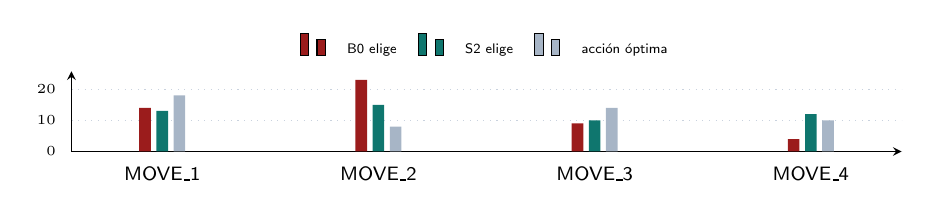
\begin{tikzpicture}
\begin{axis}[width=\linewidth, height=2.6cm, ybar, bar width=4.2pt, ymin=0,
  symbolic x coords={MOVE\_1,MOVE\_2,MOVE\_3,MOVE\_4}, xtick=data,
  xticklabel style={font=\scriptsize}, yticklabel style={font=\tiny},
  legend style={font=\tiny,at={(0.5,1.03)},anchor=south,legend columns=3,draw=none,fill=none,column sep=2mm},
  axis lines=left, tick style={draw=none}, ymajorgrids, grid style={rule,dotted},
  enlarge x limits=0.14, enlarge y limits={upper,value=0.12}]
\addplot[fill=crimson,draw=none] coordinates {\posBase};
\addplot[fill=teal,draw=none] coordinates {\posStwo};
\addplot[fill=steel!45,draw=none] coordinates {\posOpt};
\legend{B0 elige, S2 elige, acci\'on \'optima}
\end{axis}
\end{tikzpicture}\par}
\vspace{-0.8mm}
{\scriptsize \textbf{Sesgo de posici\'on:} con las 4 rotaciones de A2, B0 eligi\'o la \emph{misma casilla} en las 4 en \sameSlot\ estados y el \emph{mismo movimiento} en \sameMove\ (de \permComplete). $\chi^2$ vs uniforme: B0 \chiBase\ ($p{=}\chiPBase$), S2 \chiStwo\ ($p{=}\chiPStwo$).}

% ============================================================ 7. FALLO S2
\vspace{0.7mm}
\ifnum\hasFailure=1
\begin{failbox}{7. Caso real donde S2 falla: estado \fcId\ (\fcDiff), \fcPlayer\ vs \fcEnemy}
{\centering\scriptsize
\begin{tabular}{@{}lllcccc@{}}
& & & \multicolumn{2}{c}{\textbf{efectividad}} & \multicolumn{2}{c}{\textbf{score}}\\
& \textbf{mov.} & \textbf{tipo} & \textbf{modelo} & \textbf{Gen I} & \textbf{S2} & \textbf{real}\\
\midrule
\fcTable
\end{tabular}\par}
\vspace{0.2mm}
{\footnotesize Eligi\'o \fcChosen; el \'optimo era \fcOptimal\ (pierde el \fcRegret\,\% del mejor score). \textbf{Por qu\'e:} ante \fcAtk\,$\to$\,\fcDef\ el modelo dijo ``\fcSaid'' ($\times$\fcModel); en Gen I es $\times$\fcTruth.
\ifnum\fcIsModern=1 Es el valor de las generaciones posteriores: la tabla cambi\'o en Gen~II y el modelo no separa generaciones aunque se le pida Gen~I.\else Es un hecho de la tabla que el modelo no sabe.\fi\ Con los hechos correctos la misma calculadora acierta: \fcFixed.}
\end{failbox}
\else
\begin{failbox}{7. Caso real donde S2 falla}
\footnotesize \ph{Se completa con \texttt{python report/fill\_d2.py} tras la corrida.}
\end{failbox}
\fi

% ============================================================ 8. LIMITES
\heading{8. L\'imites conocidos}
\begin{itemize}
\item \verdictSH
\item \textbf{Por qu\'e: el modelo no sabe la tabla de tipos.} Respondi\'o ``normal damage'' en \neutralShare\ pares (\neutralPct\,\%); cuando dijo otra cosa acert\'o \nonNeutral\ (nuevos: \nonNeutralH) y llam\'o \emph{super effective} a pares del mismo tipo (\sameSuper) que en Gen~I no lo son. Responder siempre $\times$1 acierta \constOne\ pares; el modelo, \factRight/\factPairs. Por efectividad real: $\times$2 \recallTwo, $\times$1 \recallOne, $\times$0{,}5 \recallHalf, $\times$0 \recallZero. \genBullet
\item \textbf{Costo:} \callsStwo\ preguntas por estado vs 1 de B0; en la T4, \secsStwoH\ vs \secsBaseH\,s por estado (respuestas cortas; cada par se pregunta una vez). Como en el D1, solo da\~no inmediato: no usa HP, velocidad ni estados alterados.
\item \textbf{Qu\'e sigue (D3):} el cuello de botella pas\'o de \emph{combinar} a \emph{saber}: ense\~narle la tabla (ajuste fino); darla por recuperaci\'on har\'ia innecesario al modelo en este paso.
\end{itemize}
\end{minipage}

\vfill
\begin{tcolorbox}[colback=paper,colframe=navy,boxrule=0.8pt,left=2mm,right=2mm,top=0.9mm,bottom=0.9mm,arc=1mm,
  before skip=0pt,after skip=0pt]
\scriptsize \textbf{Reproducir:} \texttt{python -m d2.evaluate [-{}-holdout]} \textbullet\ \texttt{python -m d2.demo [-{}-replay \fcIdOrQ]} \textbullet\ cifras desde \texttt{results\_d2*/} con \texttt{python report/fill\_d2.py}
\end{tcolorbox}

\end{document}
